% Options for packages loaded elsewhere
% Options for packages loaded elsewhere
\PassOptionsToPackage{unicode}{hyperref}
\PassOptionsToPackage{hyphens}{url}
\PassOptionsToPackage{dvipsnames,svgnames,x11names}{xcolor}
\PassOptionsToPackage{space}{xeCJK}
%
\documentclass[
  chinese-hans,
  letterpaper,
  DIV=11,
  numbers=noendperiod]{scrartcl}
\usepackage{xcolor}
\usepackage{amsmath,amssymb}
\setcounter{secnumdepth}{5}
\usepackage{iftex}
\ifPDFTeX
  \usepackage[T1]{fontenc}
  \usepackage[utf8]{inputenc}
  \usepackage{textcomp} % provide euro and other symbols
\else % if luatex or xetex
  \usepackage{unicode-math} % this also loads fontspec
  \defaultfontfeatures{Scale=MatchLowercase}
  \defaultfontfeatures[\rmfamily]{Ligatures=TeX,Scale=1}
\fi
\usepackage{lmodern}
\ifPDFTeX\else
  % xetex/luatex font selection
  \ifXeTeX
    \usepackage{xeCJK}
    \setCJKmainfont[]{HarmonyOS Sans SC}
  \fi
  \ifLuaTeX
    \usepackage[]{luatexja-fontspec}
    \setmainjfont[]{HarmonyOS Sans SC}
  \fi
\fi
% Use upquote if available, for straight quotes in verbatim environments
\IfFileExists{upquote.sty}{\usepackage{upquote}}{}
\IfFileExists{microtype.sty}{% use microtype if available
  \usepackage[]{microtype}
  \UseMicrotypeSet[protrusion]{basicmath} % disable protrusion for tt fonts
}{}
\makeatletter
\@ifundefined{KOMAClassName}{% if non-KOMA class
  \IfFileExists{parskip.sty}{%
    \usepackage{parskip}
  }{% else
    \setlength{\parindent}{0pt}
    \setlength{\parskip}{6pt plus 2pt minus 1pt}}
}{% if KOMA class
  \KOMAoptions{parskip=half}}
\makeatother
% Make \paragraph and \subparagraph free-standing
\makeatletter
\ifx\paragraph\undefined\else
  \let\oldparagraph\paragraph
  \renewcommand{\paragraph}{
    \@ifstar
      \xxxParagraphStar
      \xxxParagraphNoStar
  }
  \newcommand{\xxxParagraphStar}[1]{\oldparagraph*{#1}\mbox{}}
  \newcommand{\xxxParagraphNoStar}[1]{\oldparagraph{#1}\mbox{}}
\fi
\ifx\subparagraph\undefined\else
  \let\oldsubparagraph\subparagraph
  \renewcommand{\subparagraph}{
    \@ifstar
      \xxxSubParagraphStar
      \xxxSubParagraphNoStar
  }
  \newcommand{\xxxSubParagraphStar}[1]{\oldsubparagraph*{#1}\mbox{}}
  \newcommand{\xxxSubParagraphNoStar}[1]{\oldsubparagraph{#1}\mbox{}}
\fi
\makeatother

\usepackage{color}
\usepackage{fancyvrb}
\newcommand{\VerbBar}{|}
\newcommand{\VERB}{\Verb[commandchars=\\\{\}]}
\DefineVerbatimEnvironment{Highlighting}{Verbatim}{commandchars=\\\{\}}
% Add ',fontsize=\small' for more characters per line
\usepackage{framed}
\definecolor{shadecolor}{RGB}{241,243,245}
\newenvironment{Shaded}{\begin{snugshade}}{\end{snugshade}}
\newcommand{\AlertTok}[1]{\textcolor[rgb]{0.68,0.00,0.00}{#1}}
\newcommand{\AnnotationTok}[1]{\textcolor[rgb]{0.37,0.37,0.37}{#1}}
\newcommand{\AttributeTok}[1]{\textcolor[rgb]{0.40,0.45,0.13}{#1}}
\newcommand{\BaseNTok}[1]{\textcolor[rgb]{0.68,0.00,0.00}{#1}}
\newcommand{\BuiltInTok}[1]{\textcolor[rgb]{0.00,0.23,0.31}{#1}}
\newcommand{\CharTok}[1]{\textcolor[rgb]{0.13,0.47,0.30}{#1}}
\newcommand{\CommentTok}[1]{\textcolor[rgb]{0.37,0.37,0.37}{#1}}
\newcommand{\CommentVarTok}[1]{\textcolor[rgb]{0.37,0.37,0.37}{\textit{#1}}}
\newcommand{\ConstantTok}[1]{\textcolor[rgb]{0.56,0.35,0.01}{#1}}
\newcommand{\ControlFlowTok}[1]{\textcolor[rgb]{0.00,0.23,0.31}{\textbf{#1}}}
\newcommand{\DataTypeTok}[1]{\textcolor[rgb]{0.68,0.00,0.00}{#1}}
\newcommand{\DecValTok}[1]{\textcolor[rgb]{0.68,0.00,0.00}{#1}}
\newcommand{\DocumentationTok}[1]{\textcolor[rgb]{0.37,0.37,0.37}{\textit{#1}}}
\newcommand{\ErrorTok}[1]{\textcolor[rgb]{0.68,0.00,0.00}{#1}}
\newcommand{\ExtensionTok}[1]{\textcolor[rgb]{0.00,0.23,0.31}{#1}}
\newcommand{\FloatTok}[1]{\textcolor[rgb]{0.68,0.00,0.00}{#1}}
\newcommand{\FunctionTok}[1]{\textcolor[rgb]{0.28,0.35,0.67}{#1}}
\newcommand{\ImportTok}[1]{\textcolor[rgb]{0.00,0.46,0.62}{#1}}
\newcommand{\InformationTok}[1]{\textcolor[rgb]{0.37,0.37,0.37}{#1}}
\newcommand{\KeywordTok}[1]{\textcolor[rgb]{0.00,0.23,0.31}{\textbf{#1}}}
\newcommand{\NormalTok}[1]{\textcolor[rgb]{0.00,0.23,0.31}{#1}}
\newcommand{\OperatorTok}[1]{\textcolor[rgb]{0.37,0.37,0.37}{#1}}
\newcommand{\OtherTok}[1]{\textcolor[rgb]{0.00,0.23,0.31}{#1}}
\newcommand{\PreprocessorTok}[1]{\textcolor[rgb]{0.68,0.00,0.00}{#1}}
\newcommand{\RegionMarkerTok}[1]{\textcolor[rgb]{0.00,0.23,0.31}{#1}}
\newcommand{\SpecialCharTok}[1]{\textcolor[rgb]{0.37,0.37,0.37}{#1}}
\newcommand{\SpecialStringTok}[1]{\textcolor[rgb]{0.13,0.47,0.30}{#1}}
\newcommand{\StringTok}[1]{\textcolor[rgb]{0.13,0.47,0.30}{#1}}
\newcommand{\VariableTok}[1]{\textcolor[rgb]{0.07,0.07,0.07}{#1}}
\newcommand{\VerbatimStringTok}[1]{\textcolor[rgb]{0.13,0.47,0.30}{#1}}
\newcommand{\WarningTok}[1]{\textcolor[rgb]{0.37,0.37,0.37}{\textit{#1}}}

\usepackage{longtable,booktabs,array}
\newcounter{none} % for unnumbered tables
\usepackage{calc} % for calculating minipage widths
% Correct order of tables after \paragraph or \subparagraph
\usepackage{etoolbox}
\makeatletter
\patchcmd\longtable{\par}{\if@noskipsec\mbox{}\fi\par}{}{}
\makeatother
% Allow footnotes in longtable head/foot
\IfFileExists{footnotehyper.sty}{\usepackage{footnotehyper}}{\usepackage{footnote}}
\makesavenoteenv{longtable}
\usepackage{graphicx}
\makeatletter
\newsavebox\pandoc@box
\newcommand*\pandocbounded[1]{% scales image to fit in text height/width
  \sbox\pandoc@box{#1}%
  \Gscale@div\@tempa{\textheight}{\dimexpr\ht\pandoc@box+\dp\pandoc@box\relax}%
  \Gscale@div\@tempb{\linewidth}{\wd\pandoc@box}%
  \ifdim\@tempb\p@<\@tempa\p@\let\@tempa\@tempb\fi% select the smaller of both
  \ifdim\@tempa\p@<\p@\scalebox{\@tempa}{\usebox\pandoc@box}%
  \else\usebox{\pandoc@box}%
  \fi%
}
% Set default figure placement to htbp
\def\fps@figure{htbp}
\makeatother



\ifLuaTeX
\usepackage[bidi=basic,shorthands=off,provide=*]{babel}
\else
\usepackage[bidi=default,shorthands=off,provide=*]{babel}
\fi
\ifLuaTeX
  \usepackage{selnolig} % disable illegal ligatures
\fi


\setlength{\emergencystretch}{3em} % prevent overfull lines

\providecommand{\tightlist}{%
  \setlength{\itemsep}{0pt}\setlength{\parskip}{0pt}}



 


\KOMAoption{captions}{tableheading}
\makeatletter
\@ifpackageloaded{tcolorbox}{}{\usepackage[skins,breakable]{tcolorbox}}
\@ifpackageloaded{fontawesome5}{}{\usepackage{fontawesome5}}
\definecolor{quarto-callout-color}{HTML}{909090}
\definecolor{quarto-callout-note-color}{HTML}{0758E5}
\definecolor{quarto-callout-important-color}{HTML}{CC1914}
\definecolor{quarto-callout-warning-color}{HTML}{EB9113}
\definecolor{quarto-callout-tip-color}{HTML}{00A047}
\definecolor{quarto-callout-caution-color}{HTML}{FC5300}
\definecolor{quarto-callout-color-frame}{HTML}{acacac}
\definecolor{quarto-callout-note-color-frame}{HTML}{4582ec}
\definecolor{quarto-callout-important-color-frame}{HTML}{d9534f}
\definecolor{quarto-callout-warning-color-frame}{HTML}{f0ad4e}
\definecolor{quarto-callout-tip-color-frame}{HTML}{02b875}
\definecolor{quarto-callout-caution-color-frame}{HTML}{fd7e14}
\makeatother
\makeatletter
\@ifpackageloaded{caption}{}{\usepackage{caption}}
\AtBeginDocument{%
\ifdefined\contentsname
  \renewcommand*\contentsname{目录}
\else
  \newcommand\contentsname{目录}
\fi
\ifdefined\listfigurename
  \renewcommand*\listfigurename{图索引}
\else
  \newcommand\listfigurename{图索引}
\fi
\ifdefined\listtablename
  \renewcommand*\listtablename{表索引}
\else
  \newcommand\listtablename{表索引}
\fi
\ifdefined\figurename
  \renewcommand*\figurename{图}
\else
  \newcommand\figurename{图}
\fi
\ifdefined\tablename
  \renewcommand*\tablename{表}
\else
  \newcommand\tablename{表}
\fi
}
\@ifpackageloaded{float}{}{\usepackage{float}}
\floatstyle{ruled}
\@ifundefined{c@chapter}{\newfloat{codelisting}{h}{lop}}{\newfloat{codelisting}{h}{lop}[chapter]}
\floatname{codelisting}{列表}
\newcommand*\listoflistings{\listof{codelisting}{列表索引}}
\makeatother
\makeatletter
\makeatother
\makeatletter
\@ifpackageloaded{caption}{}{\usepackage{caption}}
\@ifpackageloaded{subcaption}{}{\usepackage{subcaption}}
\makeatother
\usepackage{bookmark}
\IfFileExists{xurl.sty}{\usepackage{xurl}}{} % add URL line breaks if available
\urlstyle{same}
\hypersetup{
  pdftitle={中介模型},
  pdfauthor={Qingyao Zhang},
  pdflang={zh-Hans},
  colorlinks=true,
  linkcolor={blue},
  filecolor={Maroon},
  citecolor={Blue},
  urlcolor={Blue},
  pdfcreator={LaTeX via pandoc}}


\title{中介模型}
\usepackage{etoolbox}
\makeatletter
\providecommand{\subtitle}[1]{% add subtitle to \maketitle
  \apptocmd{\@title}{\par {\large #1 \par}}{}{}
}
\makeatother
\subtitle{Mediation}
\author{Qingyao Zhang}
\date{2026-04-14}
\begin{document}
\maketitle

\renewcommand*\contentsname{目录}
{
\setcounter{tocdepth}{3}
\tableofcontents
}

\begin{Shaded}
\begin{Highlighting}[numbers=left,,]
\FunctionTok{library}\NormalTok{(lavaan)}
\DocumentationTok{\#\# This is lavaan 0.6{-}21}
\DocumentationTok{\#\# lavaan is FREE software! Please report any bugs.}
\FunctionTok{data}\NormalTok{(}\StringTok{"depress"}\NormalTok{, }\AttributeTok{package =} \StringTok{"Keng"}\NormalTok{)}
\FunctionTok{library}\NormalTok{(ggplot2)}
\end{Highlighting}
\end{Shaded}

\section{回归模型}\label{ux56deux5f52ux6a21ux578b}

以depress数据为例，理论上，依恋焦虑(X)作为人格特征会影响个体的抑郁水平(Y)。

\subsection{模型图}\label{ux6a21ux578bux56fe}

依恋焦虑(X)与抑郁水平(Y)的关系可以用下面的模型图表示：

\begin{figure}[H]

{\centering 
\includegraphics[width=0.55\linewidth,height=\textheight,keepaspectratio]{../../courses/PsyEduStat/mediation/regression_simple.png}

}

\caption{简单回归}

\end{figure}%

在上图中，箭头的起点是原因，是自变量，箭头的终点是结果，是结果变量，箭头在概念上表示自变量对结果变量的效应。

\subsection{回归方程}\label{ux56deux5f52ux65b9ux7a0b}

我们可以用回归分析检验依恋焦虑(X)与抑郁水平(Y)关系，上图中的箭头与回归分析中的回归系数c对应：

\[
Y = intercept + c*X
\]

\subsection{模型估计}\label{ux6a21ux578bux4f30ux8ba1}

我们通过lavaan程序包进行上述统计分析。lavaan需要3步：

\begin{enumerate}
\def\labelenumi{\arabic{enumi}.}
\tightlist
\item
  通过字符串\texttt{""}界定统计模型，即界定变量间的关系。
\item
  通过\texttt{sem()}对统计模型进行拟合，对模型中的参数(例如：回归系数)进行估计。
\item
  通过\texttt{summary()}输出统计结果。
\end{enumerate}

具体代码如下。注意，在lavaan中，我们可以为回归系数指定标签，这相当于为回归系数起了一个名字。在下面的代码中，我们为attach\_anx对depr1的回归系数指定标签c。

\begin{Shaded}
\begin{Highlighting}[numbers=left,,]
\CommentTok{\# 界定模型}
\NormalTok{model1 }\OtherTok{\textless{}{-}} \StringTok{"}
\StringTok{  \# 为attach\_anx对depr1的回归系数指定标签c。}
\StringTok{  depr1 \textasciitilde{} c*attach\_anx}
\StringTok{"}
\CommentTok{\# 拟合模型}
\NormalTok{fit1 }\OtherTok{\textless{}{-}} \FunctionTok{sem}\NormalTok{(}
  \AttributeTok{model =}\NormalTok{ model1,}
  \AttributeTok{data =}\NormalTok{ depress,}
  \CommentTok{\# 模型包含截距}
  \AttributeTok{meanstructure =} \ConstantTok{TRUE}
\NormalTok{)}
\end{Highlighting}
\end{Shaded}

\begin{Shaded}
\begin{Highlighting}[numbers=left,,]
\CommentTok{\# 输出结果}
\FunctionTok{summary}\NormalTok{(}
\NormalTok{  fit1,}
  \CommentTok{\# 输出模型拟合指数}
  \AttributeTok{fit.measures =} \ConstantTok{TRUE}\NormalTok{,}
  \CommentTok{\# 输出标准化的估计结果}
  \AttributeTok{standardized =} \ConstantTok{TRUE}\NormalTok{,}
  \CommentTok{\# 输出R square}
  \AttributeTok{rsquare =} \ConstantTok{TRUE}
\NormalTok{)}
\end{Highlighting}
\end{Shaded}

上面的回归分析实际上是一个最简单的路径分析(path
analysis)。在路径分析中，回归系数被称为路径系数。下面我们通过注释讲解\texttt{summary()}输出的结果：

\begin{Shaded}
\begin{Highlighting}[numbers=left,,]
\CommentTok{\# lavaan进行了1次迭代即完成参数估计。需重点关注。}
\DocumentationTok{\#\# lavaan 0.6{-}21 ended normally after 1 iteration}
\CommentTok{\# 算法。该信息不重要。}
\DocumentationTok{\#\#   Estimator                                         ML}
\CommentTok{\# 参数收敛方法。该信息不重要。}
\DocumentationTok{\#\#   Optimization method                           NLMINB}
\CommentTok{\# 模型参数的数量。需重点关注。}
\DocumentationTok{\#\#   Number of model parameters                         3}
\CommentTok{\# 样本量。需重点关注。}
\DocumentationTok{\#\#                                                   Used       Total}
\DocumentationTok{\#\#   Number of observations                           174         185}
\CommentTok{\# 模型拟合程度的卡方检验。需重点关注。 }
\DocumentationTok{\#\# Model Test User Model:}
\DocumentationTok{\#\#                                                       }
\DocumentationTok{\#\#   Test statistic                                 0.000}
\DocumentationTok{\#\#   Degrees of freedom                                 0}
\CommentTok{\# 基线模型拟合程度的卡方检验。该信息不重要。}
\DocumentationTok{\#\# Model Test Baseline Model:}
\DocumentationTok{\#\# }
\DocumentationTok{\#\#  Test statistic                                 2.591}
\DocumentationTok{\#\#  Degrees of freedom                                 1}
\DocumentationTok{\#\#  P{-}value                                        0.107}
\CommentTok{\# 模型拟合指数CFI、TLI，一般要求大于0.90}
\DocumentationTok{\#\# User Model versus Baseline Model:}
\DocumentationTok{\#\# }
\DocumentationTok{\#\#   Comparative Fit Index (CFI)                    1.000}
\DocumentationTok{\#\#   Tucker{-}Lewis Index (TLI)                       1.000}
\CommentTok{\# 模型拟合指数似然值与信息准则指数AIC、BIC、SABIC，越小越好}
\DocumentationTok{\#\# Loglikelihood and Information Criteria:}
\DocumentationTok{\#\# }
\DocumentationTok{\#\#  Loglikelihood user model (H0)                {-}75.688}
\DocumentationTok{\#\#  Loglikelihood unrestricted model (H1)        {-}75.688}
\DocumentationTok{\#\#                                                      }
\DocumentationTok{\#\#  Akaike (AIC)                                 157.376}
\DocumentationTok{\#\#  Bayesian (BIC)                               166.853}
\DocumentationTok{\#\#  Sample{-}size adjusted Bayesian (SABIC)        157.353}
\CommentTok{\# 模型拟合指数RMSEA，一般要求小于0.05 }
\DocumentationTok{\#\# Root Mean Square Error of Approximation:}
\DocumentationTok{\#\# }
\DocumentationTok{\#\#   RMSEA                                          0.000}
\DocumentationTok{\#\#   90 Percent confidence interval {-} lower         0.000}
\DocumentationTok{\#\#   90 Percent confidence interval {-} upper         0.000}
\DocumentationTok{\#\#   P{-}value H\_0: RMSEA \textless{}= 0.050                       NA}
\DocumentationTok{\#\#   P{-}value H\_0: RMSEA \textgreater{}= 0.080                       NA}
\CommentTok{\# 模型拟合指数SRMR，一般要求小于0.05}
\DocumentationTok{\#\# Standardized Root Mean Square Residual:}
\DocumentationTok{\#\# }
\DocumentationTok{\#\#   SRMR                                           0.000}
\CommentTok{\# 参数估计方法。该信息不重要。}
\DocumentationTok{\#\# Parameter Estimates:}
\DocumentationTok{\#\# }
\DocumentationTok{\#\#   Standard errors                             Standard}
\DocumentationTok{\#\#   Information                                 Expected}
\DocumentationTok{\#\#   Information saturated (h1) model          Structured}
\CommentTok{\# 回归系数及其z检验。 }
\CommentTok{\# Std.lv为将潜变量进行标准化的估计结果，该信息不重要。}
\CommentTok{\# Std.all为将自变量、结果变量、潜变量进行标准化的估计结果。}
\CommentTok{\# Std.all包含了我们需要的标准化路径系数。}
\DocumentationTok{\#\# Regressions:}
\DocumentationTok{\#\#                    Estimate  Std.Err  z{-}value  P(\textgreater{}|z|)   Std.lv  Std.all}
\CommentTok{\# 输出结果也标明了attach\_anx对depr1的回归系数的标签c}
\DocumentationTok{\#\#  depr1 \textasciitilde{}                                                               }
\DocumentationTok{\#\#     attach\_anx (c)    0.037    0.023    1.616    0.106    0.037    0.122}
\CommentTok{\# depr1的截距}
\DocumentationTok{\#\# Intercepts:}
\DocumentationTok{\#\#                    Estimate  Std.Err  z{-}value  P(\textgreater{}|z|)   Std.lv  Std.all}
\DocumentationTok{\#\#    .depr1             1.842    0.058   31.997    0.000    1.842    4.891}
\CommentTok{\# depr1的残差的方差, \textasciigrave{}.depr1\textasciigrave{}表示depr1的残差}
\DocumentationTok{\#\# Variances:}
\DocumentationTok{\#\#                    Estimate  Std.Err  z{-}value  P(\textgreater{}|z|)   Std.lv  Std.all}
\DocumentationTok{\#\#    .depr1             0.140    0.015    9.327    0.000    0.140    0.985}
\CommentTok{\# 以depr1为结果变量的回归方程的R{-}Square}
\DocumentationTok{\#\# R{-}Square:}
\DocumentationTok{\#\#                    Estimate}
\DocumentationTok{\#\#     depr1             0.015}
\end{Highlighting}
\end{Shaded}

上述结果表明，依恋焦虑对抑郁的效应是0.037，\emph{p} = 0.106。

\section{中介模型}\label{ux4e2dux4ecbux6a21ux578b}

依恋焦虑是如何影响抑郁的？理论上，依恋焦虑会影响个体的情绪应对，情绪应对继而会影响抑郁。换句话说，依恋焦虑会通过影响情绪应对间接地影响抑郁，情绪应对是依恋焦虑影响抑郁的路径、桥梁、机制，情绪应对是依恋焦虑与抑郁之间的中介。

\subsection{模型图}\label{ux6a21ux578bux56fe-1}

依恋焦虑、情绪应对、抑郁的关系可以用下面的模型图表示：

\begin{figure}[H]

{\centering 
\includegraphics[width=0.55\linewidth,height=\textheight,keepaspectratio]{../../courses/PsyEduStat/mediation/mediation_simple.png}

}

\caption{简单中介}

\end{figure}%

在上图中，X经过M影响Y，这构成了一条因果链。

\subsection{回归方程}\label{ux56deux5f52ux65b9ux7a0b-1}

上面的模型图包含两个回归方程。一个是以M为结果变量的回归方程，另一个是以Y为结果变量的回归方程：

\begin{align}
M &= intercept + a*X \\
Y &= intercept + b*M + c^{'}*X
\end{align}

\begin{tcolorbox}[enhanced jigsaw, arc=.35mm, bottomrule=.15mm, bottomtitle=1mm, breakable, colback=white, colbacktitle=quarto-callout-tip-color!10!white, colframe=quarto-callout-tip-color-frame, coltitle=black, left=2mm, leftrule=.75mm, opacityback=0, opacitybacktitle=0.6, rightrule=.15mm, title=\textcolor{quarto-callout-tip-color}{\faLightbulb}\hspace{0.5em}{如何根据模型图写回归方程}, titlerule=0mm, toprule=.15mm, toptitle=1mm]

回归方程中的结果变量与自变量由箭头\textbf{直接}相连。

\begin{enumerate}
\def\labelenumi{\arabic{enumi}.}
\tightlist
\item
  先确定结果变量，箭头所指为结果变量。结果变量的数量等于回归方程的数量。
\item
  再沿着箭头逆向回溯每个结果变量的自变量，箭头来源为自变量。
\end{enumerate}

\end{tcolorbox}

\subsection{直接效应、间接效应与总效应}\label{ux76f4ux63a5ux6548ux5e94ux95f4ux63a5ux6548ux5e94ux4e0eux603bux6548ux5e94}

根据上面的模型图，依恋焦虑对抑郁的效应可以分成两部分：

\begin{enumerate}
\def\labelenumi{\arabic{enumi}.}
\tightlist
\item
  依恋焦虑直接对抑郁产生的直接效应(direct effect)。
\item
  依恋焦虑经情绪应对方式对抑郁产生的间接效应(indirect effect)。
\end{enumerate}

自变量对结果变量的效应可以用回归系数来量化。那么，依恋焦虑对抑郁的直接效应与间接效应具体是多少？依恋焦虑对抑郁的直接效应为c'，c'为X的偏回归系数。依恋焦虑经情绪应对方式对抑郁的间接效应为回归系数a与b的乘积ab。如何理解间接效应？回归系数a是X对M的效应，X变化一个单位会导致M变化a个单位；回归系数b是M对Y的偏回归系数，M变化一个单位会导致Y变化b个单位；那么，X变化1个单位会通过M间接地导致Y变化几个单位呢？a*b个单位，因此X经M影响Y的间接效应为a*b。依恋焦虑对抑郁的总效应为直接效应与间接效应的和c'+a*b。

\subsection{模型估计}\label{ux6a21ux578bux4f30ux8ba1-1}

路径分析又被称为``同时回归分析''，意即，路径分析能够同时进行多个回归分析，因此，路径分析适合用来检验中介模型。下面我们通过lavaan检验上述中介模型。为了检验间接效应，我们在界定模型时除了界定两个回归方程，还需要：

\begin{itemize}
\tightlist
\item
  为回归系数a与b打标签；
\item
  使用a与b定义一个新的统计量I表示间接效应；
\item
  使用a、b、c'定义一个新的统计量T表示总效应。
\end{itemize}

\begin{Shaded}
\begin{Highlighting}[numbers=left,,]
\NormalTok{model2 }\OtherTok{\textless{}{-}} \StringTok{"}
\StringTok{  cope\_emo1 \textasciitilde{} a*attach\_anx}
\StringTok{  \# 为与c区分，我们在代码中用cc表示c\textquotesingle{}}
\StringTok{  depr1 \textasciitilde{} b*cope\_emo1 + cc*attach\_anx}
\StringTok{  \# 间接效应}
\StringTok{  I := a*b}
\StringTok{  T := a*b + cc}
\StringTok{"}
\CommentTok{\# 拟合模型}
\NormalTok{fit2 }\OtherTok{\textless{}{-}} \FunctionTok{sem}\NormalTok{(}
  \AttributeTok{model =}\NormalTok{ model2,}
  \AttributeTok{data =}\NormalTok{ depress,}
  \CommentTok{\# 模型包含截距}
  \AttributeTok{meanstructure =} \ConstantTok{TRUE}
\NormalTok{)}
\CommentTok{\# 输出结果}
\FunctionTok{summary}\NormalTok{(}
\NormalTok{  fit2,}
  \CommentTok{\# 输出模型拟合指数}
  \AttributeTok{fit.measures =} \ConstantTok{TRUE}\NormalTok{,}
  \CommentTok{\# 输出标准化的估计结果}
  \AttributeTok{standardized =} \ConstantTok{TRUE}\NormalTok{,}
  \CommentTok{\# 输出R square}
  \AttributeTok{rsquare =} \ConstantTok{TRUE}
\NormalTok{)}
\DocumentationTok{\#\# lavaan 0.6{-}21 ended normally after 1 iteration}
\DocumentationTok{\#\# }
\DocumentationTok{\#\#   Estimator                                         ML}
\DocumentationTok{\#\#   Optimization method                           NLMINB}
\DocumentationTok{\#\#   Number of model parameters                         7}
\DocumentationTok{\#\# }
\DocumentationTok{\#\#                                                   Used       Total}
\DocumentationTok{\#\#   Number of observations                           174         185}
\DocumentationTok{\#\# }
\DocumentationTok{\#\# Model Test User Model:}
\DocumentationTok{\#\#                                                       }
\DocumentationTok{\#\#   Test statistic                                 0.000}
\DocumentationTok{\#\#   Degrees of freedom                                 0}
\DocumentationTok{\#\# }
\DocumentationTok{\#\# Model Test Baseline Model:}
\DocumentationTok{\#\# }
\DocumentationTok{\#\#   Test statistic                                37.105}
\DocumentationTok{\#\#   Degrees of freedom                                 3}
\DocumentationTok{\#\#   P{-}value                                        0.000}
\DocumentationTok{\#\# }
\DocumentationTok{\#\# User Model versus Baseline Model:}
\DocumentationTok{\#\# }
\DocumentationTok{\#\#   Comparative Fit Index (CFI)                    1.000}
\DocumentationTok{\#\#   Tucker{-}Lewis Index (TLI)                       1.000}
\DocumentationTok{\#\# }
\DocumentationTok{\#\# Loglikelihood and Information Criteria:}
\DocumentationTok{\#\# }
\DocumentationTok{\#\#   Loglikelihood user model (H0)               {-}237.498}
\DocumentationTok{\#\#   Loglikelihood unrestricted model (H1)       {-}237.498}
\DocumentationTok{\#\#                                                       }
\DocumentationTok{\#\#   Akaike (AIC)                                 488.996}
\DocumentationTok{\#\#   Bayesian (BIC)                               511.109}
\DocumentationTok{\#\#   Sample{-}size adjusted Bayesian (SABIC)        488.943}
\DocumentationTok{\#\# }
\DocumentationTok{\#\# Root Mean Square Error of Approximation:}
\DocumentationTok{\#\# }
\DocumentationTok{\#\#   RMSEA                                          0.000}
\DocumentationTok{\#\#   90 Percent confidence interval {-} lower         0.000}
\DocumentationTok{\#\#   90 Percent confidence interval {-} upper         0.000}
\DocumentationTok{\#\#   P{-}value H\_0: RMSEA \textless{}= 0.050                       NA}
\DocumentationTok{\#\#   P{-}value H\_0: RMSEA \textgreater{}= 0.080                       NA}
\DocumentationTok{\#\# }
\DocumentationTok{\#\# Standardized Root Mean Square Residual:}
\DocumentationTok{\#\# }
\DocumentationTok{\#\#   SRMR                                           0.000}
\DocumentationTok{\#\# }
\DocumentationTok{\#\# Parameter Estimates:}
\DocumentationTok{\#\# }
\DocumentationTok{\#\#   Standard errors                             Standard}
\DocumentationTok{\#\#   Information                                 Expected}
\DocumentationTok{\#\#   Information saturated (h1) model          Structured}
\DocumentationTok{\#\# }
\DocumentationTok{\#\# Regressions:}
\DocumentationTok{\#\#                    Estimate  Std.Err  z{-}value  P(\textgreater{}|z|)   Std.lv  Std.all}
\DocumentationTok{\#\#   cope\_emo1 \textasciitilde{}                                                           }
\DocumentationTok{\#\#     attach\_nx  (a)    0.088    0.041    2.136    0.033    0.088    0.160}
\DocumentationTok{\#\#   depr1 \textasciitilde{}                                                               }
\DocumentationTok{\#\#     cope\_emo1  (b)    0.223    0.039    5.723    0.000    0.223    0.400}
\DocumentationTok{\#\#     attach\_nx (cc)    0.018    0.021    0.823    0.410    0.018    0.058}
\DocumentationTok{\#\# }
\DocumentationTok{\#\# Intercepts:}
\DocumentationTok{\#\#                    Estimate  Std.Err  z{-}value  P(\textgreater{}|z|)   Std.lv  Std.all}
\DocumentationTok{\#\#    .cope\_emo1         2.405    0.103   23.360    0.000    2.405    3.551}
\DocumentationTok{\#\#    .depr1             1.307    0.107   12.167    0.000    1.307    3.470}
\DocumentationTok{\#\# }
\DocumentationTok{\#\# Variances:}
\DocumentationTok{\#\#                    Estimate  Std.Err  z{-}value  P(\textgreater{}|z|)   Std.lv  Std.all}
\DocumentationTok{\#\#    .cope\_emo1         0.447    0.048    9.327    0.000    0.447    0.974}
\DocumentationTok{\#\#    .depr1             0.118    0.013    9.327    0.000    0.118    0.829}
\DocumentationTok{\#\# }
\DocumentationTok{\#\# R{-}Square:}
\DocumentationTok{\#\#                    Estimate}
\DocumentationTok{\#\#     cope\_emo1         0.026}
\DocumentationTok{\#\#     depr1             0.171}
\DocumentationTok{\#\# }
\DocumentationTok{\#\# Defined Parameters:}
\DocumentationTok{\#\#                    Estimate  Std.Err  z{-}value  P(\textgreater{}|z|)   Std.lv  Std.all}
\DocumentationTok{\#\#     I                 0.020    0.010    2.001    0.045    0.020    0.064}
\DocumentationTok{\#\#     T                 0.037    0.023    1.616    0.106    0.037    0.122}
\end{Highlighting}
\end{Shaded}

对于上述统计结果中的大部分内容，前文已作过解释，此处不再赘述。

我们关心的问题是：依恋焦虑经情绪应对影响抑郁的机制真的存在吗？情绪应对在依恋焦虑与抑郁之间起中介作用吗？要回答上述问题，我们需要对间接效应的显著性进行检验？若间接效应显著，则证明间接效应不等于0，即间接效应是存在的，情绪应对在依恋焦虑与抑郁之间起中介作用。

如何判断间接效应是否显著？最简单的方法是依次检验法，所谓依次检验法就是先看中介路径的前半路径a是否显著，再看中介路径的后半路径b是否显著，如果a与b都显著，就意味着a与b都不等于0，如果a与b都不等于0，那么a与b的乘积一定不等于0。从上面的结果可以看出，前半路径a不显著。到这里，我们是否可以得出结论``间接效应不显著''呢？不可以。依次检验法虽然简单，但是该方法统计检验力低。当a与b中有至少一个系数不显著时，我们不能直接下结论``间接效应不显著''，而是应当采用更可靠的方法进一步对间接效应进行检验。

在上面的结果中，我们能够看到最后两行对I与T进行了z检验，这里的z检验被称为\textbf{delta检验}或者\textbf{sobel检验}。与依次检验法不同，delta检验并非对a与b两个系数分别作检验，而是对它们的乘积(也就是间接效应)直接进行检验。从lavaan的结果可以看出，I不显著，T不显著。到这里，我们是否可以得出结论``间接效应不显著''呢？不可以。研究表明，虽然\textbf{delta检验}的统计检验力高于依次检验法，但依然低于bootstrap法。

\subsection{通过bootstrap法检验间接效应}\label{ux901aux8fc7bootstrapux6cd5ux68c0ux9a8cux95f4ux63a5ux6548ux5e94}

什么是bootstrap法？简言之，bootstrap法是对真实抽样过程的模拟。显著性检验的本质是将统计量放在抽样分布中，继而判断统计量的极端程度。但是，现实情况是我们无法从总体中进行抽样。bootstrap法的逻辑就是用实际样本代替总体，从样本本身进行{有放回的}取样。这种取样被称为自取样，bootstrap法也称为自举法。以depress数据为例，我们可以通过有放回的取样从depress数据中抽取1000个样本量为94的bootstrap样本，每个bootstrap样本都可以计算得到一个间接效应值I，我们总计将得到1000个间接效应估计值I，这1000个I就构成了I的bootstrap分布，我们用bootstrap分布近似的代替I的抽样分布。如此一来，我们就可以用bootstrap分布的95\%置信区间判断实际间接效应I的显著性。该置信区间被称为bootstrap
95\% 百分位置信区间。若I的bootstrap 95\%
百分位置信区间\textbf{包含0}，那么I与0没有显著差异，即间接效应不显著；若I的bootstrap
95\%
百分位置信区间\textbf{不包含0}，那么I与0没有显著差异，即间接效应显著。

在检验间接效应的显著性时，我们并不需要手动进行bootstrap取样的过程，R语言可以自动完成这个过程，并将我们需要的bootstrap
95\%
百分位置信区间告诉我们。若要在lavaan中使用bootstrap法检验间接效应，我们需要在\texttt{sem()}函数中指定参数\texttt{se\ =\ "boot"}，并指定bootstrap取样的次数(至少1000)，\texttt{bootstrap\ =\ 1000}。同时，为了能获知模型参数的置信区间，我们需要在\texttt{summary()}函数中指定参数\texttt{ci\ =\ TRUE}。

\begin{Shaded}
\begin{Highlighting}[numbers=left,,]
\NormalTok{fit3 }\OtherTok{\textless{}{-}} \FunctionTok{sem}\NormalTok{(}
  \AttributeTok{model =}\NormalTok{ model2,}
  \AttributeTok{data =}\NormalTok{ depress,}
  \CommentTok{\# 模型包含截距}
  \AttributeTok{meanstructure =} \ConstantTok{TRUE}\NormalTok{,}
  \CommentTok{\# 使用bootstrap方法计算标准误}
  \AttributeTok{se =} \StringTok{"boot"}\NormalTok{,}
  \CommentTok{\# 指定bootstrap取样的次数为1000}
  \AttributeTok{bootstrap =} \DecValTok{1000}\NormalTok{,}
  \CommentTok{\# 通过并行计算加快计算，该参数可省略}
  \AttributeTok{parallel =} \StringTok{"snow"}
\NormalTok{)}
\end{Highlighting}
\end{Shaded}

\begin{Shaded}
\begin{Highlighting}[numbers=left,,]
\CommentTok{\# 输出结果}
\FunctionTok{summary}\NormalTok{(}
\NormalTok{  fit3,}
  \CommentTok{\# 简化输出}
  \AttributeTok{fit.measures =} \ConstantTok{FALSE}\NormalTok{,}
  \CommentTok{\# 输出置信区间}
  \AttributeTok{ci =} \ConstantTok{TRUE}\NormalTok{,}
  \CommentTok{\# 简化输出}
  \AttributeTok{standardized =} \ConstantTok{FALSE}\NormalTok{,}
  \CommentTok{\# 简化输出}
  \AttributeTok{rsquare =} \ConstantTok{FALSE}
\NormalTok{)}
\DocumentationTok{\#\# lavaan 0.6{-}21 ended normally after 1 iteration}
\DocumentationTok{\#\# }
\DocumentationTok{\#\#   Estimator                                         ML}
\DocumentationTok{\#\#   Optimization method                           NLMINB}
\DocumentationTok{\#\#   Number of model parameters                         7}
\DocumentationTok{\#\# }
\DocumentationTok{\#\#                                                   Used       Total}
\DocumentationTok{\#\#   Number of observations                           174         185}
\DocumentationTok{\#\# }
\DocumentationTok{\#\# Model Test User Model:}
\DocumentationTok{\#\#                                                       }
\DocumentationTok{\#\#   Test statistic                                 0.000}
\DocumentationTok{\#\#   Degrees of freedom                                 0}
\DocumentationTok{\#\# }
\DocumentationTok{\#\# Parameter Estimates:}
\DocumentationTok{\#\# }
\DocumentationTok{\#\#   Standard errors                            Bootstrap}
\DocumentationTok{\#\#   Number of requested bootstrap draws             1000}
\DocumentationTok{\#\#   Number of successful bootstrap draws            1000}
\DocumentationTok{\#\# }
\DocumentationTok{\#\# Regressions:}
\DocumentationTok{\#\#                    Estimate  Std.Err  z{-}value  P(\textgreater{}|z|) ci.lower ci.upper}
\DocumentationTok{\#\#   cope\_emo1 \textasciitilde{}                                                           }
\DocumentationTok{\#\#     attach\_nx  (a)    0.088    0.045    1.944    0.052   {-}0.001    0.177}
\DocumentationTok{\#\#   depr1 \textasciitilde{}                                                               }
\DocumentationTok{\#\#     cope\_emo1  (b)    0.223    0.040    5.591    0.000    0.142    0.301}
\DocumentationTok{\#\#     attach\_nx (cc)    0.018    0.023    0.758    0.448   {-}0.026    0.065}
\DocumentationTok{\#\# }
\DocumentationTok{\#\# Intercepts:}
\DocumentationTok{\#\#                    Estimate  Std.Err  z{-}value  P(\textgreater{}|z|) ci.lower ci.upper}
\DocumentationTok{\#\#    .cope\_emo1         2.405    0.110   21.961    0.000    2.190    2.622}
\DocumentationTok{\#\#    .depr1             1.307    0.106   12.338    0.000    1.094    1.507}
\DocumentationTok{\#\# }
\DocumentationTok{\#\# Variances:}
\DocumentationTok{\#\#                    Estimate  Std.Err  z{-}value  P(\textgreater{}|z|) ci.lower ci.upper}
\DocumentationTok{\#\#    .cope\_emo1         0.447    0.042   10.526    0.000    0.369    0.535}
\DocumentationTok{\#\#    .depr1             0.118    0.012   10.057    0.000    0.094    0.141}
\DocumentationTok{\#\# }
\DocumentationTok{\#\# Defined Parameters:}
\DocumentationTok{\#\#                    Estimate  Std.Err  z{-}value  P(\textgreater{}|z|) ci.lower ci.upper}
\DocumentationTok{\#\#     I                 0.020    0.010    1.884    0.060   {-}0.000    0.042}
\DocumentationTok{\#\#     T                 0.037    0.025    1.479    0.139   {-}0.013    0.087}
\end{Highlighting}
\end{Shaded}

上述结果表明，间接效应与总效应不显著，95\% CI = {[}-0.012,
0.044{]}，95\% CI = {[}-0.030, 0.094{]}。

有些研究者建议使用偏差校正的bootstrap百分位置信区间，我们可以在\texttt{parameterEstimates()}中设置参数\texttt{boot.ci.type\ =\ "bca.simple"}来得到这种置信区间结果：

\begin{Shaded}
\begin{Highlighting}[numbers=left,,]
\FunctionTok{parameterEstimates}\NormalTok{(}
\NormalTok{  fit3,}
  \AttributeTok{zstat =} \ConstantTok{FALSE}\NormalTok{,}
  \AttributeTok{pvalue =} \ConstantTok{FALSE}\NormalTok{,}
  \AttributeTok{boot.ci.type =} \StringTok{"bca.simple"}
\NormalTok{)}
\DocumentationTok{\#\#           lhs op        rhs label   est    se ci.lower ci.upper}
\DocumentationTok{\#\# 1   cope\_emo1  \textasciitilde{} attach\_anx     a 0.088 0.045    0.000    0.178}
\DocumentationTok{\#\# 2       depr1  \textasciitilde{}  cope\_emo1     b 0.223 0.040    0.144    0.302}
\DocumentationTok{\#\# 3       depr1  \textasciitilde{} attach\_anx    cc 0.018 0.023   {-}0.030    0.063}
\DocumentationTok{\#\# 4   cope\_emo1 \textasciitilde{}\textasciitilde{}  cope\_emo1       0.447 0.042    0.377    0.547}
\DocumentationTok{\#\# 5       depr1 \textasciitilde{}\textasciitilde{}      depr1       0.118 0.012    0.100    0.147}
\DocumentationTok{\#\# 6  attach\_anx \textasciitilde{}\textasciitilde{} attach\_anx       1.512 0.000    1.512    1.512}
\DocumentationTok{\#\# 7   cope\_emo1 \textasciitilde{}1                  2.405 0.110    2.179    2.612}
\DocumentationTok{\#\# 8       depr1 \textasciitilde{}1                  1.307 0.106    1.093    1.504}
\DocumentationTok{\#\# 9  attach\_anx \textasciitilde{}1                  2.174 0.000    2.174    2.174}
\DocumentationTok{\#\# 10          I :=        a*b     I 0.020 0.010    0.002    0.045}
\DocumentationTok{\#\# 11          T :=     a*b+cc     T 0.037 0.025   {-}0.014    0.086}
\end{Highlighting}
\end{Shaded}

上述结果表明，间接效应与总效应不显著，95\% CI = {[}-0.008,
0.043{]}，95\% CI = {[}-0.026, 0.094{]}。

\subsection{bootstrap分布}\label{bootstrapux5206ux5e03}

为了进一步理解bootstrap法，我们通过\texttt{bootstrapLavaan()}函数来演示bootstrap法的过程。在下面的代码中，\texttt{bootstrapLavaan()}函数从样本量为94的depress数据中进行有放回的取样，获取1000个样本量为94的bootstrap样本。每一个样本都可以对中介模型进行估计，得到自己的一套参数估计值，这些参数估计值存储在resamples中。

\begin{Shaded}
\begin{Highlighting}[numbers=left,,]
\NormalTok{resamples }\OtherTok{\textless{}{-}} \FunctionTok{bootstrapLavaan}\NormalTok{(}
\NormalTok{  fit3,}
  \AttributeTok{R =} \DecValTok{1000}\NormalTok{L,}
  \AttributeTok{FUN =} \StringTok{"coef"}\NormalTok{,}
  \AttributeTok{parallel =} \StringTok{"snow"}
\NormalTok{)}
\end{Highlighting}
\end{Shaded}

接下来，我们计算中介效应I，我们将得到1000个bootstrap样本的1000个I。这1000个I就构成了I的bootstrap分布，这个分布基本上以实际样本的I的估计值0.015为中心。

\begin{Shaded}
\begin{Highlighting}[numbers=left,,]
\NormalTok{resamples }\OtherTok{\textless{}{-}} \FunctionTok{as.data.frame}\NormalTok{(resamples)}
\NormalTok{resamples}\SpecialCharTok{$}\NormalTok{I }\OtherTok{\textless{}{-}}\NormalTok{  resamples}\SpecialCharTok{$}\NormalTok{a}\SpecialCharTok{*}\NormalTok{resamples}\SpecialCharTok{$}\NormalTok{b}
\FunctionTok{ggplot}\NormalTok{(resamples, }\FunctionTok{aes}\NormalTok{(I)) }\SpecialCharTok{+}
  \FunctionTok{geom\_histogram}\NormalTok{(}\AttributeTok{fill =} \StringTok{"wheat"}\NormalTok{)}
\DocumentationTok{\#\# \textasciigrave{}stat\_bin()\textasciigrave{} using \textasciigrave{}bins = 30\textasciigrave{}. Pick better value \textasciigrave{}binwidth\textasciigrave{}.}
\end{Highlighting}
\end{Shaded}

\pandocbounded{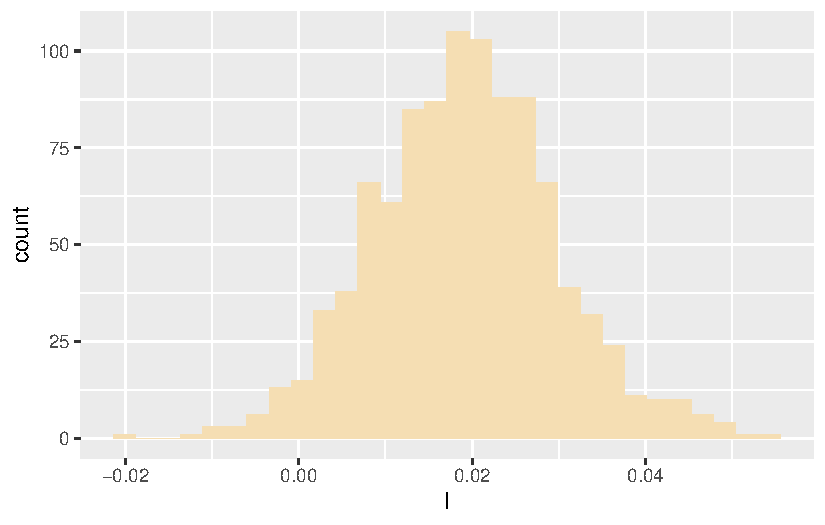
\includegraphics[keepaspectratio]{index_files/figure-pdf/unnamed-chunk-8-1.pdf}}

我们通过quantile()函数计算bootstrap分布的95\%百分位置信区间：

\begin{Shaded}
\begin{Highlighting}[numbers=left,,]
\NormalTok{CI }\OtherTok{\textless{}{-}} \FunctionTok{quantile}\NormalTok{(resamples}\SpecialCharTok{$}\NormalTok{I, }\FunctionTok{c}\NormalTok{(}\FloatTok{0.025}\NormalTok{, }\FloatTok{0.975}\NormalTok{))}
\NormalTok{CI}
\DocumentationTok{\#\#          2.5\%         97.5\% }
\DocumentationTok{\#\# {-}0.0008999375  0.0420967640}
\end{Highlighting}
\end{Shaded}

我们可以将实际样本的I的估计值与95\%置信区间标注在上述分布图中：

\begin{Shaded}
\begin{Highlighting}[numbers=left,,]
\NormalTok{CI }\OtherTok{\textless{}{-}} \FunctionTok{round}\NormalTok{(CI, }\DecValTok{3}\NormalTok{)}
\FunctionTok{names}\NormalTok{(CI) }\OtherTok{\textless{}{-}} \ConstantTok{NULL}
\FunctionTok{ggplot}\NormalTok{(resamples, }\FunctionTok{aes}\NormalTok{(I)) }\SpecialCharTok{+}
  \FunctionTok{geom\_histogram}\NormalTok{(}\AttributeTok{fill =} \StringTok{"wheat"}\NormalTok{) }\SpecialCharTok{+}
  \FunctionTok{geom\_vline}\NormalTok{(}\AttributeTok{xintercept =} \FloatTok{0.015}\NormalTok{) }\SpecialCharTok{+}
  \FunctionTok{geom\_vline}\NormalTok{(}\AttributeTok{xintercept =}\NormalTok{ CI, }\AttributeTok{color =} \StringTok{"brown"}\NormalTok{) }\SpecialCharTok{+}
  \FunctionTok{scale\_x\_continuous}\NormalTok{(}\AttributeTok{breaks =} \FunctionTok{c}\NormalTok{(CI, }\DecValTok{0}\NormalTok{, }\FloatTok{0.015}\NormalTok{))}
\DocumentationTok{\#\# \textasciigrave{}stat\_bin()\textasciigrave{} using \textasciigrave{}bins = 30\textasciigrave{}. Pick better value \textasciigrave{}binwidth\textasciigrave{}.}
\end{Highlighting}
\end{Shaded}

\pandocbounded{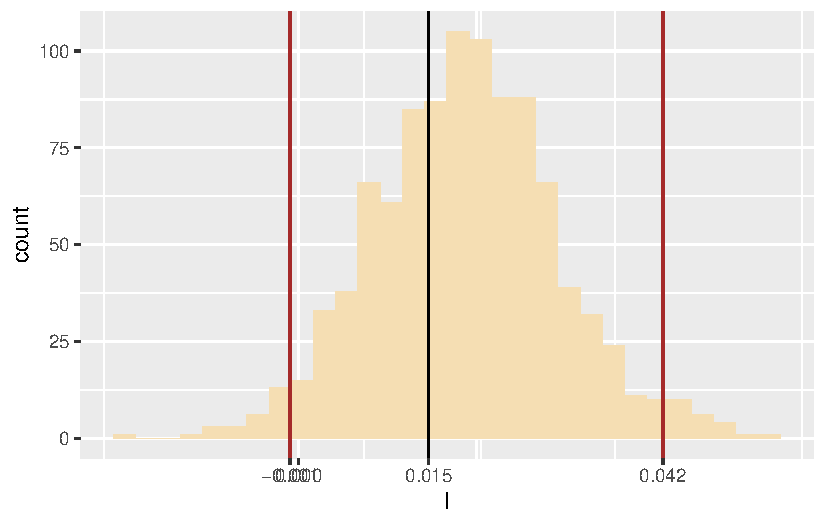
\includegraphics[keepaspectratio]{index_files/figure-pdf/unnamed-chunk-10-1.pdf}}

可见，I的bootstrap 95\% 百分位置信区间包含0，即I不显著。

\section{多重中介模型}\label{ux591aux91cdux4e2dux4ecbux6a21ux578b}

一般情况下，自变量影响结果变量的路径会有多条，即中介变量有多个，这就形成了多重中介模型。根据中介变量之间的关系，多重中介模型又可以分为并行中介、链式中介、复合式中介。

\begin{itemize}
\tightlist
\item
  并行中介：多个中介变量呈并列关系。
\item
  链式中介：多个中介变量共同构成因果链。
\item
  复合式中介：在多个中介变量中，部分变量呈并列关系，部分变量构成因果链。
\end{itemize}

例如，假定X与Y之间有两个中介变量M1与M2，链式中介的模型图见下方：

\begin{figure}[H]

{\centering 
\includegraphics[width=0.75\linewidth,height=\textheight,keepaspectratio]{../../courses/PsyEduStat/mediation/mediation_serial.png}

}

\caption{链式多重中介}

\end{figure}%

与简单中介模型，多重中介模型的统计分析并没有增加多少难度。建立多重中介模型只需注意两点：

\begin{enumerate}
\def\labelenumi{\arabic{enumi}.}
\tightlist
\item
  先根据假设绘制模型图，再根据模型图写出所有回归方程。
\item
  定义并检验特定间接效应、总间接效应、总效应。
\end{enumerate}

多重中介模型中的中介路径(因果链)有多个，我们需要对每一条中介路径的特定间接效应进行检验，不要遗漏。从因果链的起点开始，到因果链的终点结束，这条中介路径上的所有回归系数(路径系数)的积就是这条路径的特定间接效应。特定间接效应的和为总间接效应，总间接效应与直接效应的和为总效应。

\subsection{链式多重中介}\label{ux94feux5f0fux591aux91cdux4e2dux4ecb}

\subsubsection{模型图}\label{ux6a21ux578bux56fe-2}

以depress数据为例，前文考察了依恋焦虑经情绪应对方式影响抑郁的简单中介模型，这里进一步考察：性别(X)经依恋焦虑(M1)、情绪应对方式(M2)影响抑郁(Y)的多重中介模型，这里假设四个变量之间的关系符合下方链式多重中介模型：

\begin{figure}[H]

{\centering 
\includegraphics[width=0.75\linewidth,height=\textheight,keepaspectratio]{../../courses/PsyEduStat/mediation/mediation_serial2.png}

}

\caption{链式多重中介}

\end{figure}%

\subsubsection{回归方程}\label{ux56deux5f52ux65b9ux7a0b-2}

该模型中的结果变量有三个：M1、M2、Y。这三个结果变量的回归方程分别是：

\begin{align}
M1 &= intercept + s1*X \\
M2 &= intercept + s4*X +  s2*M1 \\
Y &= intercept + s6*X + s5*M1 + s3*M2
\end{align}

\subsubsection{直接效应、间接效应与总效应}\label{ux76f4ux63a5ux6548ux5e94ux95f4ux63a5ux6548ux5e94ux4e0eux603bux6548ux5e94-1}

上述多重中介模型的直接效应、间接效应、总效应如下：

\begin{longtable}[]{@{}llll@{}}
\caption{三种效应}\tabularnewline
\toprule\noalign{}
效应 & 标签 & 路径 & 计算 \\
\midrule\noalign{}
\endfirsthead
\toprule\noalign{}
效应 & 标签 & 路径 & 计算 \\
\midrule\noalign{}
\endhead
\bottomrule\noalign{}
\endlastfoot
直接效应 & D & x --\textgreater{} Y & s6 \\
特定间接效应 & I1 & x --\textgreater{} M1 --\textgreater{} Y & s1*s5 \\
特定间接效应 & I2 & x --\textgreater{} M2 --\textgreater{} Y & s4*s3 \\
特定间接效应 & I3 & x --\textgreater{} M1 --\textgreater{} M2
--\textgreater{} Y & s1*s2*s3 \\
总间接效应 & I & & I1+I2+I3 \\
总效应 & T & & T=I+D \\
\end{longtable}

\subsubsection{模型估计}\label{ux6a21ux578bux4f30ux8ba1-2}

与简单中介模型相比，多重中介模型的代码不过是多了几个回归方程、多了几个自定义的统计量。在下面的代码中，我们按照前文的模型图与表格为相应的路径系数打上标签，并定义直接效应、间接效应与总效应。

\begin{Shaded}
\begin{Highlighting}[numbers=left,,]
\NormalTok{model4 }\OtherTok{\textless{}{-}} \StringTok{"}
\StringTok{  \# M1的回归方程，为路径系数指定标签s1}
\StringTok{  attach\_anx \textasciitilde{} s1*gender}
\StringTok{  \# M2的回归方程，为路径系数指定标签s4、s2}
\StringTok{  cope\_emo1 \textasciitilde{} s4*gender + s2*attach\_anx}
\StringTok{  \# Y的回归方程，为路径系数指定标签s6、s5、s3}
\StringTok{  depr1 \textasciitilde{} s6*gender + s5*attach\_anx + s3*cope\_emo1}
\StringTok{  \# 间接效应}
\StringTok{  D := s6}
\StringTok{  I1 := s1*s5}
\StringTok{  I2 := s4*s3}
\StringTok{  I3 := s1*s2*s3}
\StringTok{  I := I1+I2+I3}
\StringTok{  T := I+D}
\StringTok{"}
\CommentTok{\# 拟合模型}
\NormalTok{fit4 }\OtherTok{\textless{}{-}} \FunctionTok{sem}\NormalTok{(}
  \AttributeTok{model =}\NormalTok{ model4,}
  \AttributeTok{data =}\NormalTok{ depress,}
  \CommentTok{\# 模型包含截距}
  \AttributeTok{meanstructure =} \ConstantTok{TRUE}\NormalTok{,}
  \CommentTok{\# 使用bootstrap方法计算标准误}
  \AttributeTok{se =} \StringTok{"boot"}\NormalTok{,}
  \CommentTok{\# 指定bootstrap取样的次数为1000}
  \AttributeTok{bootstrap =} \DecValTok{1000}\NormalTok{,}
  \CommentTok{\# 通过并行计算加快计算，该参数可省略}
  \AttributeTok{parallel =} \StringTok{"snow"}
\NormalTok{)}
\CommentTok{\# 输出结果}
\FunctionTok{summary}\NormalTok{(}
\NormalTok{  fit4,}
  \CommentTok{\# 拟合指数}
  \AttributeTok{fit.measures =} \ConstantTok{TRUE}\NormalTok{,}
  \CommentTok{\# 输出置信区间}
  \AttributeTok{ci =} \ConstantTok{TRUE}\NormalTok{,}
  \CommentTok{\# 简化输出}
  \AttributeTok{standardized =} \ConstantTok{FALSE}\NormalTok{,}
  \CommentTok{\# 简化输出}
  \AttributeTok{rsquare =} \ConstantTok{FALSE}
\NormalTok{)}
\DocumentationTok{\#\# lavaan 0.6{-}21 ended normally after 1 iteration}
\DocumentationTok{\#\# }
\DocumentationTok{\#\#   Estimator                                         ML}
\DocumentationTok{\#\#   Optimization method                           NLMINB}
\DocumentationTok{\#\#   Number of model parameters                        12}
\DocumentationTok{\#\# }
\DocumentationTok{\#\#                                                   Used       Total}
\DocumentationTok{\#\#   Number of observations                           174         185}
\DocumentationTok{\#\# }
\DocumentationTok{\#\# Model Test User Model:}
\DocumentationTok{\#\#                                                       }
\DocumentationTok{\#\#   Test statistic                                 0.000}
\DocumentationTok{\#\#   Degrees of freedom                                 0}
\DocumentationTok{\#\# }
\DocumentationTok{\#\# Model Test Baseline Model:}
\DocumentationTok{\#\# }
\DocumentationTok{\#\#   Test statistic                                39.999}
\DocumentationTok{\#\#   Degrees of freedom                                 6}
\DocumentationTok{\#\#   P{-}value                                        0.000}
\DocumentationTok{\#\# }
\DocumentationTok{\#\# User Model versus Baseline Model:}
\DocumentationTok{\#\# }
\DocumentationTok{\#\#   Comparative Fit Index (CFI)                    1.000}
\DocumentationTok{\#\#   Tucker{-}Lewis Index (TLI)                       1.000}
\DocumentationTok{\#\# }
\DocumentationTok{\#\# Loglikelihood and Information Criteria:}
\DocumentationTok{\#\# }
\DocumentationTok{\#\#   Loglikelihood user model (H0)               {-}518.901}
\DocumentationTok{\#\#   Loglikelihood unrestricted model (H1)       {-}518.901}
\DocumentationTok{\#\#                                                       }
\DocumentationTok{\#\#   Akaike (AIC)                                1061.802}
\DocumentationTok{\#\#   Bayesian (BIC)                              1099.710}
\DocumentationTok{\#\#   Sample{-}size adjusted Bayesian (SABIC)       1061.711}
\DocumentationTok{\#\# }
\DocumentationTok{\#\# Root Mean Square Error of Approximation:}
\DocumentationTok{\#\# }
\DocumentationTok{\#\#   RMSEA                                          0.000}
\DocumentationTok{\#\#   90 Percent confidence interval {-} lower         0.000}
\DocumentationTok{\#\#   90 Percent confidence interval {-} upper         0.000}
\DocumentationTok{\#\#   P{-}value H\_0: RMSEA \textless{}= 0.050                       NA}
\DocumentationTok{\#\#   P{-}value H\_0: RMSEA \textgreater{}= 0.080                       NA}
\DocumentationTok{\#\# }
\DocumentationTok{\#\# Standardized Root Mean Square Residual:}
\DocumentationTok{\#\# }
\DocumentationTok{\#\#   SRMR                                           0.000}
\DocumentationTok{\#\# }
\DocumentationTok{\#\# Parameter Estimates:}
\DocumentationTok{\#\# }
\DocumentationTok{\#\#   Standard errors                            Bootstrap}
\DocumentationTok{\#\#   Number of requested bootstrap draws             1000}
\DocumentationTok{\#\#   Number of successful bootstrap draws            1000}
\DocumentationTok{\#\# }
\DocumentationTok{\#\# Regressions:}
\DocumentationTok{\#\#                    Estimate  Std.Err  z{-}value  P(\textgreater{}|z|) ci.lower ci.upper}
\DocumentationTok{\#\#   attach\_anx \textasciitilde{}                                                          }
\DocumentationTok{\#\#     gender    (s1)    0.121    0.187    0.647    0.518   {-}0.261    0.498}
\DocumentationTok{\#\#   cope\_emo1 \textasciitilde{}                                                           }
\DocumentationTok{\#\#     gender    (s4)    0.159    0.103    1.540    0.124   {-}0.045    0.361}
\DocumentationTok{\#\#     attach\_nx (s2)    0.085    0.043    1.988    0.047   {-}0.003    0.166}
\DocumentationTok{\#\#   depr1 \textasciitilde{}                                                               }
\DocumentationTok{\#\#     gender    (s6)    0.010    0.055    0.185    0.853   {-}0.100    0.114}
\DocumentationTok{\#\#     attach\_nx (s5)    0.018    0.023    0.755    0.450   {-}0.025    0.069}
\DocumentationTok{\#\#     cope\_emo1 (s3)    0.222    0.039    5.620    0.000    0.145    0.299}
\DocumentationTok{\#\# }
\DocumentationTok{\#\# Intercepts:}
\DocumentationTok{\#\#                    Estimate  Std.Err  z{-}value  P(\textgreater{}|z|) ci.lower ci.upper}
\DocumentationTok{\#\#    .attach\_anx        1.998    0.280    7.125    0.000    1.468    2.551}
\DocumentationTok{\#\#    .cope\_emo1         2.181    0.173   12.607    0.000    1.833    2.500}
\DocumentationTok{\#\#    .depr1             1.295    0.117   11.062    0.000    1.041    1.509}
\DocumentationTok{\#\# }
\DocumentationTok{\#\# Variances:}
\DocumentationTok{\#\#                    Estimate  Std.Err  z{-}value  P(\textgreater{}|z|) ci.lower ci.upper}
\DocumentationTok{\#\#    .attach\_anx        1.508    0.159    9.511    0.000    1.190    1.839}
\DocumentationTok{\#\#    .cope\_emo1         0.441    0.044   10.012    0.000    0.348    0.518}
\DocumentationTok{\#\#    .depr1             0.118    0.012    9.869    0.000    0.091    0.139}
\DocumentationTok{\#\# }
\DocumentationTok{\#\# Defined Parameters:}
\DocumentationTok{\#\#                    Estimate  Std.Err  z{-}value  P(\textgreater{}|z|) ci.lower ci.upper}
\DocumentationTok{\#\#     D                 0.010    0.055    0.185    0.853   {-}0.100    0.114}
\DocumentationTok{\#\#     I1                0.002    0.006    0.346    0.730   {-}0.008    0.018}
\DocumentationTok{\#\#     I2                0.035    0.025    1.430    0.153   {-}0.009    0.089}
\DocumentationTok{\#\#     I3                0.002    0.004    0.526    0.599   {-}0.005    0.013}
\DocumentationTok{\#\#     I                 0.040    0.026    1.510    0.131   {-}0.008    0.096}
\DocumentationTok{\#\#     T                 0.050    0.058    0.858    0.391   {-}0.061    0.162}
\end{Highlighting}
\end{Shaded}

上述结果表明：

\begin{longtable}[]{@{}
  >{\raggedright\arraybackslash}p{(\linewidth - 8\tabcolsep) * \real{0.1905}}
  >{\raggedright\arraybackslash}p{(\linewidth - 8\tabcolsep) * \real{0.0635}}
  >{\raggedright\arraybackslash}p{(\linewidth - 8\tabcolsep) * \real{0.3492}}
  >{\raggedright\arraybackslash}p{(\linewidth - 8\tabcolsep) * \real{0.1587}}
  >{\raggedright\arraybackslash}p{(\linewidth - 8\tabcolsep) * \real{0.2381}}@{}}
\caption{三种效应的置信区间}\tabularnewline
\toprule\noalign{}
\begin{minipage}[b]{\linewidth}\raggedright
效应
\end{minipage} & \begin{minipage}[b]{\linewidth}\raggedright
标签
\end{minipage} & \begin{minipage}[b]{\linewidth}\raggedright
路径
\end{minipage} & \begin{minipage}[b]{\linewidth}\raggedright
计算
\end{minipage} & \begin{minipage}[b]{\linewidth}\raggedright
bootstrap 95\% 百分位置信区间
\end{minipage} \\
\midrule\noalign{}
\endfirsthead
\toprule\noalign{}
\begin{minipage}[b]{\linewidth}\raggedright
效应
\end{minipage} & \begin{minipage}[b]{\linewidth}\raggedright
标签
\end{minipage} & \begin{minipage}[b]{\linewidth}\raggedright
路径
\end{minipage} & \begin{minipage}[b]{\linewidth}\raggedright
计算
\end{minipage} & \begin{minipage}[b]{\linewidth}\raggedright
bootstrap 95\% 百分位置信区间
\end{minipage} \\
\midrule\noalign{}
\endhead
\bottomrule\noalign{}
\endlastfoot
直接效应 & D & x --\textgreater{} Y & s6 & {[}-0.131, 0.158{]} \\
特定间接效应 & I1 & x --\textgreater{} M1 --\textgreater{} Y & s1*s5 &
{[}-0.040, 0.017{]} \\
特定间接效应 & I2 & x --\textgreater{} M2 --\textgreater{} Y & s4*s3 &
{[}-0.107, 0.025{]} \\
特定间接效应 & I3 & x --\textgreater{} M1 --\textgreater{} M2
--\textgreater{} Y & s1*s2*s3 & {[}-0.023, 0.005{]} \\
总间接效应 & I & & I1+I2+I3 & {[}-0.123, 0.024{]} \\
总效应 & T & & T=I+D & {[}-0.185, 0.122{]} \\
\end{longtable}

\subsection{并行多重中介模型}\label{ux5e76ux884cux591aux91cdux4e2dux4ecbux6a21ux578b}

以depress数据为例，前文考察了依恋焦虑经情绪应对方式影响抑郁的简单中介模型，这里我们进一步考察依恋焦虑经三种应对方式问题应对、情绪应对、回避应对影响抑郁的并行多重中介模型。

\subsubsection{模型图}\label{ux6a21ux578bux56fe-3}

四个变量的模型图如下：

\begin{figure}[H]

{\centering 
\includegraphics[width=0.55\linewidth,height=\textheight,keepaspectratio]{../../courses/PsyEduStat/mediation/mediation_parallel.png}

}

\caption{并行多重中介}

\end{figure}%

注意，理论上该模型中三种应对方式的关系是并列的，即，它们相互之前没有因果之分。但是，三种应对方式是相关还是不相关呢？事物是普遍联系的，中介变量之间大概率是相关的。上面的模型图事实上省略了三个中介变量两两之间的相关关系，更严谨的做法是通过双向箭头将这种相关关系表达出来。

\subsubsection{回归方程}\label{ux56deux5f52ux65b9ux7a0b-3}

回归方程比较简单，这里不再赘述。

\subsubsection{直接效应、间接效应与总效应}\label{ux76f4ux63a5ux6548ux5e94ux95f4ux63a5ux6548ux5e94ux4e0eux603bux6548ux5e94-2}

三种效应的计算比较简单，这里不再赘述。

\subsubsection{模型估计}\label{ux6a21ux578bux4f30ux8ba1-3}

\begin{Shaded}
\begin{Highlighting}[numbers=left,,]
\NormalTok{model5 }\OtherTok{\textless{}{-}} \StringTok{"}
\StringTok{  \# M1的回归方程，为路径系数指定标签}
\StringTok{  cope\_task1 \textasciitilde{} a1*attach\_anx}
\StringTok{  \# M2的回归方程，为路径系数指定标签}
\StringTok{  cope\_emo1 \textasciitilde{} a2*attach\_anx}
\StringTok{  \# M3的回归方程，为路径系数指定标签}
\StringTok{  cope\_avo1 \textasciitilde{} a3*attach\_anx}
\StringTok{  \# Y的回归方程，为路径系数指定标签}
\StringTok{  depr1 \textasciitilde{} b1*cope\_task1 + b2*cope\_emo1 + b3*cope\_avo1 + cc*attach\_anx}
\StringTok{  \# 相关}
\StringTok{  cope\_task1 \textasciitilde{}\textasciitilde{} cope\_emo1 + cope\_avo1}
\StringTok{  cope\_emo1 \textasciitilde{}\textasciitilde{} cope\_avo1}
\StringTok{  \# 间接效应}
\StringTok{  D := cc}
\StringTok{  I1 := a1*b1}
\StringTok{  I2 := a2*b2}
\StringTok{  I3 := a3*b3}
\StringTok{  I := I1+I2+I3}
\StringTok{  T := I+D}
\StringTok{"}
\CommentTok{\# 拟合模型}
\NormalTok{fit5 }\OtherTok{\textless{}{-}} \FunctionTok{sem}\NormalTok{(}
  \AttributeTok{model =}\NormalTok{ model5,}
  \AttributeTok{data =}\NormalTok{ depress,}
  \CommentTok{\# 模型包含截距}
  \AttributeTok{meanstructure =} \ConstantTok{TRUE}\NormalTok{,}
  \CommentTok{\# 使用bootstrap方法计算标准误}
  \AttributeTok{se =} \StringTok{"boot"}\NormalTok{,}
  \CommentTok{\# 指定bootstrap取样的次数为1000}
  \AttributeTok{bootstrap =} \DecValTok{1000}\NormalTok{,}
  \CommentTok{\# 通过并行计算加快计算，该参数可省略}
  \AttributeTok{parallel =} \StringTok{"snow"}
\NormalTok{)}
\CommentTok{\# 输出结果}
\FunctionTok{summary}\NormalTok{(}
\NormalTok{  fit5,}
  \CommentTok{\# 拟合指数}
  \AttributeTok{fit.measures =} \ConstantTok{TRUE}\NormalTok{,}
  \CommentTok{\# 输出置信区间}
  \AttributeTok{ci =} \ConstantTok{TRUE}\NormalTok{,}
  \CommentTok{\# 输出标准化系数}
  \AttributeTok{standardized =} \ConstantTok{TRUE}\NormalTok{,}
  \CommentTok{\# 简化输出}
  \AttributeTok{rsquare =} \ConstantTok{FALSE}
\NormalTok{)}
\DocumentationTok{\#\# lavaan 0.6{-}21 ended normally after 22 iterations}
\DocumentationTok{\#\# }
\DocumentationTok{\#\#   Estimator                                         ML}
\DocumentationTok{\#\#   Optimization method                           NLMINB}
\DocumentationTok{\#\#   Number of model parameters                        18}
\DocumentationTok{\#\# }
\DocumentationTok{\#\#                                                   Used       Total}
\DocumentationTok{\#\#   Number of observations                           174         185}
\DocumentationTok{\#\# }
\DocumentationTok{\#\# Model Test User Model:}
\DocumentationTok{\#\#                                                       }
\DocumentationTok{\#\#   Test statistic                                 0.000}
\DocumentationTok{\#\#   Degrees of freedom                                 0}
\DocumentationTok{\#\# }
\DocumentationTok{\#\# Model Test Baseline Model:}
\DocumentationTok{\#\# }
\DocumentationTok{\#\#   Test statistic                                92.979}
\DocumentationTok{\#\#   Degrees of freedom                                10}
\DocumentationTok{\#\#   P{-}value                                        0.000}
\DocumentationTok{\#\# }
\DocumentationTok{\#\# User Model versus Baseline Model:}
\DocumentationTok{\#\# }
\DocumentationTok{\#\#   Comparative Fit Index (CFI)                    1.000}
\DocumentationTok{\#\#   Tucker{-}Lewis Index (TLI)                       1.000}
\DocumentationTok{\#\# }
\DocumentationTok{\#\# Loglikelihood and Information Criteria:}
\DocumentationTok{\#\# }
\DocumentationTok{\#\#   Loglikelihood user model (H0)               {-}548.838}
\DocumentationTok{\#\#   Loglikelihood unrestricted model (H1)       {-}548.838}
\DocumentationTok{\#\#                                                       }
\DocumentationTok{\#\#   Akaike (AIC)                                1133.676}
\DocumentationTok{\#\#   Bayesian (BIC)                              1190.539}
\DocumentationTok{\#\#   Sample{-}size adjusted Bayesian (SABIC)       1133.540}
\DocumentationTok{\#\# }
\DocumentationTok{\#\# Root Mean Square Error of Approximation:}
\DocumentationTok{\#\# }
\DocumentationTok{\#\#   RMSEA                                          0.000}
\DocumentationTok{\#\#   90 Percent confidence interval {-} lower         0.000}
\DocumentationTok{\#\#   90 Percent confidence interval {-} upper         0.000}
\DocumentationTok{\#\#   P{-}value H\_0: RMSEA \textless{}= 0.050                       NA}
\DocumentationTok{\#\#   P{-}value H\_0: RMSEA \textgreater{}= 0.080                       NA}
\DocumentationTok{\#\# }
\DocumentationTok{\#\# Standardized Root Mean Square Residual:}
\DocumentationTok{\#\# }
\DocumentationTok{\#\#   SRMR                                           0.000}
\DocumentationTok{\#\# }
\DocumentationTok{\#\# Parameter Estimates:}
\DocumentationTok{\#\# }
\DocumentationTok{\#\#   Standard errors                            Bootstrap}
\DocumentationTok{\#\#   Number of requested bootstrap draws             1000}
\DocumentationTok{\#\#   Number of successful bootstrap draws            1000}
\DocumentationTok{\#\# }
\DocumentationTok{\#\# Regressions:}
\DocumentationTok{\#\#                    Estimate  Std.Err  z{-}value  P(\textgreater{}|z|) ci.lower ci.upper}
\DocumentationTok{\#\#   cope\_task1 \textasciitilde{}                                                          }
\DocumentationTok{\#\#     attach\_nx (a1)   {-}0.033    0.043   {-}0.768    0.442   {-}0.122    0.049}
\DocumentationTok{\#\#   cope\_emo1 \textasciitilde{}                                                           }
\DocumentationTok{\#\#     attach\_nx (a2)    0.088    0.043    2.066    0.039    0.002    0.171}
\DocumentationTok{\#\#   cope\_avo1 \textasciitilde{}                                                           }
\DocumentationTok{\#\#     attach\_nx (a3)    0.076    0.037    2.024    0.043    0.005    0.149}
\DocumentationTok{\#\#   depr1 \textasciitilde{}                                                               }
\DocumentationTok{\#\#     cope\_tsk1 (b1)   {-}0.193    0.035   {-}5.496    0.000   {-}0.258   {-}0.122}
\DocumentationTok{\#\#     cope\_emo1 (b2)    0.222    0.038    5.847    0.000    0.152    0.304}
\DocumentationTok{\#\#     cope\_avo1 (b3)   {-}0.102    0.041   {-}2.495    0.013   {-}0.179   {-}0.020}
\DocumentationTok{\#\#     attach\_nx (cc)    0.019    0.020    0.944    0.345   {-}0.018    0.062}
\DocumentationTok{\#\#    Std.lv  Std.all}
\DocumentationTok{\#\#                   }
\DocumentationTok{\#\#    {-}0.033   {-}0.058}
\DocumentationTok{\#\#                   }
\DocumentationTok{\#\#     0.088    0.160}
\DocumentationTok{\#\#                   }
\DocumentationTok{\#\#     0.076    0.159}
\DocumentationTok{\#\#                   }
\DocumentationTok{\#\#    {-}0.193   {-}0.360}
\DocumentationTok{\#\#     0.222    0.399}
\DocumentationTok{\#\#    {-}0.102   {-}0.158}
\DocumentationTok{\#\#     0.019    0.062}
\DocumentationTok{\#\# }
\DocumentationTok{\#\# Covariances:}
\DocumentationTok{\#\#                    Estimate  Std.Err  z{-}value  P(\textgreater{}|z|) ci.lower ci.upper}
\DocumentationTok{\#\#  .cope\_task1 \textasciitilde{}\textasciitilde{}                                                         }
\DocumentationTok{\#\#    .cope\_emo1        {-}0.054    0.036   {-}1.477    0.140   {-}0.127    0.024}
\DocumentationTok{\#\#    .cope\_avo1         0.011    0.032    0.335    0.737   {-}0.051    0.075}
\DocumentationTok{\#\#  .cope\_emo1 \textasciitilde{}\textasciitilde{}                                                          }
\DocumentationTok{\#\#    .cope\_avo1         0.098    0.029    3.353    0.001    0.039    0.152}
\DocumentationTok{\#\#    Std.lv  Std.all}
\DocumentationTok{\#\#                   }
\DocumentationTok{\#\#    {-}0.054   {-}0.115}
\DocumentationTok{\#\#     0.011    0.026}
\DocumentationTok{\#\#                   }
\DocumentationTok{\#\#     0.098    0.254}
\DocumentationTok{\#\# }
\DocumentationTok{\#\# Intercepts:}
\DocumentationTok{\#\#                    Estimate  Std.Err  z{-}value  P(\textgreater{}|z|) ci.lower ci.upper}
\DocumentationTok{\#\#    .cope\_task1        3.251    0.105   31.014    0.000    3.046    3.462}
\DocumentationTok{\#\#    .cope\_emo1         2.405    0.100   24.136    0.000    2.208    2.603}
\DocumentationTok{\#\#    .cope\_avo1         2.510    0.092   27.347    0.000    2.334    2.692}
\DocumentationTok{\#\#    .depr1             2.191    0.176   12.420    0.000    1.807    2.506}
\DocumentationTok{\#\#    Std.lv  Std.all}
\DocumentationTok{\#\#     3.251    4.630}
\DocumentationTok{\#\#     2.405    3.551}
\DocumentationTok{\#\#     2.510    4.283}
\DocumentationTok{\#\#     2.191    5.818}
\DocumentationTok{\#\# }
\DocumentationTok{\#\# Variances:}
\DocumentationTok{\#\#                    Estimate  Std.Err  z{-}value  P(\textgreater{}|z|) ci.lower ci.upper}
\DocumentationTok{\#\#    .cope\_task1        0.491    0.045   11.014    0.000    0.395    0.577}
\DocumentationTok{\#\#    .cope\_emo1         0.447    0.044   10.102    0.000    0.357    0.531}
\DocumentationTok{\#\#    .cope\_avo1         0.335    0.037    9.143    0.000    0.262    0.405}
\DocumentationTok{\#\#    .depr1             0.095    0.010    9.442    0.000    0.073    0.112}
\DocumentationTok{\#\#    Std.lv  Std.all}
\DocumentationTok{\#\#     0.491    0.997}
\DocumentationTok{\#\#     0.447    0.974}
\DocumentationTok{\#\#     0.335    0.975}
\DocumentationTok{\#\#     0.095    0.673}
\DocumentationTok{\#\# }
\DocumentationTok{\#\# Defined Parameters:}
\DocumentationTok{\#\#                    Estimate  Std.Err  z{-}value  P(\textgreater{}|z|) ci.lower ci.upper}
\DocumentationTok{\#\#     D                 0.019    0.020    0.944    0.345   {-}0.018    0.062}
\DocumentationTok{\#\#     I1                0.006    0.008    0.757    0.449   {-}0.009    0.025}
\DocumentationTok{\#\#     I2                0.020    0.010    1.901    0.057    0.000    0.041}
\DocumentationTok{\#\#     I3               {-}0.008    0.005   {-}1.482    0.138   {-}0.021    0.000}
\DocumentationTok{\#\#     I                 0.018    0.014    1.276    0.202   {-}0.009    0.048}
\DocumentationTok{\#\#     T                 0.037    0.025    1.489    0.137   {-}0.011    0.091}
\DocumentationTok{\#\#    Std.lv  Std.all}
\DocumentationTok{\#\#     0.019    0.062}
\DocumentationTok{\#\#     0.006    0.021}
\DocumentationTok{\#\#     0.020    0.064}
\DocumentationTok{\#\#    {-}0.008   {-}0.025}
\DocumentationTok{\#\#     0.018    0.059}
\DocumentationTok{\#\#     0.037    0.122}
\end{Highlighting}
\end{Shaded}

上述结果中出现了一部分新的内容（见下方）。这部分内容报告了三个中介变量的残差的协方差，例如，cope\_emo1的残差与cope\_avo1的残差的协方差为0.102。协方差是相关系数吗?一般不是。标准化的协方差(Std.all这一列)恰恰是相关系数。可见，cope\_emo1的残差与cope\_avo1的残差的相关系数为0.263，p
=
0.008。该结果表明，cope\_emo1的残差与cope\_avo1的残差的相关关系(协方差，相关系数)有必要保留在模型中，否则，模型拟合程度会下降，模型拟合指数会变差。

\begin{Shaded}
\begin{Highlighting}[numbers=left,,]
\DocumentationTok{\#\# Covariances:}
\DocumentationTok{\#\#                    Estimate  Std.Err  z{-}value  P(\textgreater{}|z|) ci.lower ci.upper   Std.lv  Std.all}
\DocumentationTok{\#\#  .cope\_task1 \textasciitilde{}\textasciitilde{}}
\DocumentationTok{\#\#    .cope\_emo1              {-}0.097    0.048   {-}2.025    0.043   {-}0.187    0.003   {-}0.097   {-}0.210}
\DocumentationTok{\#\#    .cope\_avo1               0.014    0.041    0.339    0.735   {-}0.068    0.095    0.014    0.033}
\DocumentationTok{\#\#  .cope\_emo1 \textasciitilde{}\textasciitilde{}}
\DocumentationTok{\#\#    .cope\_avo1               0.102    0.038    2.662    0.008    0.028    0.179    0.102    0.263}
\end{Highlighting}
\end{Shaded}

\section{模型评价}\label{ux6a21ux578bux8bc4ux4ef7}

模型拟合指数(e.g., CFI, TLI, RMSEA,
SRMR)的作用是评估模型与数据的拟合程度。理论上，若统计模型符合实际数据中变量之间的关系，模型拟合会较好。反之，若统计模型不符合实际数据中变量之间的关系，模型拟合会较差；若模型拟合会极差，模型将无法收敛，无法成功迭代，模型参数无法被估计出来，lavaan会直接输出WARNING。

如前文所示，路径分析的模型拟合一般都很好。若你的路径分析结果显示模型拟合不好，这一般是因为你遗漏了某些变量间关系(单向箭头或者双向箭头)------假设M1与M2之间存在显著的关系，但若model没有将这种关系界定出来，lavaan会理解为M1与M2之间相关为0，故模型拟合会变差。

\section{包含多自变量、多结果变量的中介模型}\label{ux5305ux542bux591aux81eaux53d8ux91cfux591aux7ed3ux679cux53d8ux91cfux7684ux4e2dux4ecbux6a21ux578b}

与SPSS中的PROCESS等统计工具相比，lavaan功能更为全面。我们可以通过lavaan检验包含多自变量、多结果变量的中介模型。事实上，只要你有数据，你可以检验你能想象到的任何一种中介模型。以depress数据为例，我们可以考察两个自变量依恋焦虑(X1)、依恋回避(X2)通过三种应对方式问题应对(M1)、情绪应对(M2)、回避应对(M2)影响两个结果变量抑郁T1(Y1)、抑郁T2(Y2)的多重中介模型。

\subsection{模型图}\label{ux6a21ux578bux56fe-4}

上述模型的模型图如下，该模型图省略了自变量之间的相关(双向箭头)、中介变量之间的相关(双向箭头)、结果变量之间的相关(双向箭头)。

\begin{figure}[H]

{\centering 
\includegraphics[width=0.55\linewidth,height=\textheight,keepaspectratio]{../../courses/PsyEduStat/mediation/mediation_IVsDVs.png}

}

\caption{包含多自变量、多结果变量的中介模型}

\end{figure}%

读者可以自己尝试检验这个模型，本文不再赘述。

全文到此结束。




\end{document}
